\chapter[Tecnoloxías Utilizadas]{
  \label{chp:tecnologia}
  Tecnoloxía
}
\minitoc
\newpage

Neste capítulo, presentanse as linguaxes, ferramentas e frameworks utilizados no desenvolvemento deste proxecto. Á hora de elixir o uso destas ferramentas valorouse a súa natureza de código aberto xa que se pretende que o resultado dispoña dunha licenza de software libre compatible coa definición da Free Software Foundation. 

Tamén se valoraron, dado que nos capítulos anteriores se insistiu na importancia dos dispositivos móbiles, no consumo da radio a través de Internet, as posibilidades de ditas ferramentas de ofrecer un bo resultado en distintos dispositivos e distintas plataformas software. 


\begin{figure}[H]
	\centering
	\includegraphics[scale=0.55,keepaspectratio=true]{./images/diagrama_tech.png}
	\caption{Diagrama de interacción de tecnoloxías.}
	\label{fig:img_diagrama_tech}
\end{figure}


\section{Linguaxes}

\subsection{Python}
\label{python}
Python é unha linguaxe de propósito xeral de alto nivel. Trátase dunha linguaxe interpretada polo que é necesario 
ter un intérprete para executar o código. Ao ser o intérprete unha capa intermedia de software entre o programa
e o sistema, Python é unha linguaxe doadamente portable entre dispositivos de distinta natureza.

A súa sintaxe baseada na indentación está pensada para favorecer a comprensión entre distintos desenvolvedores e 
facilitar o mantemento do código. 

O seu sistema de tipado implícito e a súa riqueza de bibliotecas para executar comandos de consola de xeito programático
fan que sexa moitas veces descrito coma \say{unha linguaxe de scripting orientada a obxectos}\cite{python1}, o cal serve coma 
mostra da súa flexibilidade, un dos motivos polo que foi elixida para este proxecto.

\subsubsection{Anaconda}

Anaconda é unha distribución de Python, libre e de código aberto (licenza BSD), utilizada normalmente para análise estatística e machine learning. Inclúe, ademais dunha completa instalación do intérprete de Python, un rico conxunto de librarías de uso común e o xestor de paquetes conda, sendo esas dúas últimas melloras o motivo primordial polo que foi a elección para este proxecto. Conda utiliza os paquetes da comunidade de Conda Forge \cite{anaconda1}

Anaconda é responsabilidade de Anaconda Incorporated, antigo Continuum Analytics.

A versión utilizada foi a Anaconda 4.4.0 de 64 bits para Python 3, a máis nova no momento de comezar o traballo. Inclúe o intérprete para Python versión 3.6.1.


\subsection{HTML}

HTML (abreviación de HyperText Markup Language) é a linguaxe estándar para a creación da estrutura das páxinas web. Os 
elementos presentes decláranse mediante bloques representados por etiquetas(tags), de aí que reciba o nome de
\say{markup language} (linguaxe de marcado). Estas etiquetas son interpretadas polos navegadores para renderizar os 
contidos\cite{html1}. 

A estrutura declarada no código HTML pode ser representada pola interface de DOM (Document Object Model), como se amosa na figura \ref{fig:img_DOM}. O DOM é unha árbore creada polo navegador ao cargar a páxina e é moi útil para acceder aos elementos da páxina de xeito programático, como veremos máis adiante.

\begin{figure}[h]
	\centering
	\includegraphics[scale=0.7,keepaspectratio=true]{./images/DOM.png}
	\caption{Exemplo de árbore HTML DOM\protect\cite{dom}}
	\label{fig:img_DOM}
\end{figure}

Dada a natureza multimedia da web realizada, utilizouse HTML5. Esta quinta revisión do estándar inclúe novas etiquetas 
para o tratamento das imaxes e dos contidos de audio e vídeo sen necesidade de utilizar outras tecnoloxías complementarias, 
simplificando así o desenvolvemento e o mantemento posterior do portal. Desde decembro do pasado ano 2017, a versión 5.2 é a última estable recomendada polo World Wide Web Consortium(W3C)\cite{html_w3c}.

Ao ser o uso de HTML un estándar tan lonxevo, consolidado e popular, non se consideraron alternativas para este proxecto.


\subsection{CSS}

CSS (Abreviatura de Cascading Style Sheets) ou \say{Follas de estilo} é unha linguaxe empregada para definir a estética dos elementos definidos anteriormente no código HTML: A súa cor, fonte, posición... Ao separar o estilo da estrutura, favorécese a reutilización de código xa que un mesmo ficheiro de CSS pode ser utilizado en diversas páxinas ao mesmo tempo. CSS permite tamén adaptar o contido das páxinas a dispositivos de distinto tamaño\cite{css_w3c}.

\subsubsection{CSS Grid}
\label{cssgrid}

O módulo de \say{Grid} úsase para definir un deseño de interface gráfica consistente nunha cuadrícula de dúas dimensións en CSS. Nun modelo deste tipo, declárase un conxunto de elementos no HTML coma pertencentes a un \say{grid container}(contedor da grella ou da cuadrícula) e, á súa vez, zonas fillas que tomarán posición dentro dese contedor dependendo das características coas que este último fose definido na folla de estilos.

Unha cela nun contedor pode, á súa vez, consistir nun contedor en sí mesma, permitindo así deseños asimétricos. O tamaño das celas pode ser fixo, relativo á páxina ou automático dependendo do contido da cela. Por todo o dito, este módulo proporciona un nivel de flexibilidade superior ao que poderíamos obter utilizando outras alternativas populares coma CSS Flexbox. 

O nivel primeiro de CSS Grid non acadou aínda, na data de entrega desta memoria, o status de \say{recomendación} da  World Wide Web Consortium(W3C)\cite{css_grid_w3c}, porén, xa é soportado polas últimas versións dos navegadores máis populares\cite{css_grid_w3c2} polo que non se considerou un risco utilizalo neste proxecto.

\subsection{JavaScript}

JavaScript é unha linguaxe de scripting interpretada e de alto nivel. Utilízase principalmente (e tamén neste proxecto) coma unha ferramenta para mellorar a interacción coa interface web ao permitir executar código orientado a eventos no lado do cliente, aforrando recargas da páxina e incluso accesos innecesarios á base de datos xa que permite o uso do disco local mediante cookies. 

A pesares do seu nome, non garda relación algunha coa linguxe Java e serven a propósitos claramente distintos. O núcleo desta linguaxe está regulado polo estándar ECMAScript\textregistered, na súa 8\textsuperscript{a} versión\cite{ecma} no momento de entregar esta memoria. 

Como se comentou no apartado \ref{python}, que sexa interpretada implica a necesidade dun intérprete para executar o código. Ese intérprete, comunmente chamado JavaScript Engine preséntase embebido nos navegadores web. Non obstante, non existe unha única implementación senón que distintos navegadores presentan distintas versións. Para o desenvolvemento deste proxecto utilizáronse os navegadores Mozilla Firefox 57.0.1 e Google Chrome 66.0, cuxos motores de JavaScript son SpiderMonkey e V8 respectivamente\cite{javascript1}, ambos os dous libres e de código aberto.

Pese a que o seu uso nos navegadores continúa a ser a principal razón de ser desta linguaxe, tamén se utiliza a día de hoxe noutro tipo de produtos coma Node.js(para correr JavaScript no lado do servidor) ou Apache Couch DB (Para o manexo de bases de datos na nube)\cite{javascript2} 

Ademais do código en JavaScript puro, este proxecto tamén fai uso nalgunhas partes do código de funcións de jQuery.

\subsubsection{jQuery}
\label{jquery}
JQuery é unha biblioteca de JavaScript creada co fin de simplificar o \say{scripting} no lado do cliente. Trátase dunha ferramenta libre, publicada baixo licenza MIT e é mantida pola comunidade jQuery Team. No 2015, xa era empregada polo 63\% do Top Million Websites\cite{jquery}, incluíndo sitios populares coma Netflix, Amazon ou Microsoft. O seu uso segue a ser moi xeralizado a día de hoxe.  

Cunha API funcional e válida en gran parte dos navegadores web, evita moitos dos problemas de incompatibilidade que aparecen ao utilizar JavaScript puro e o código resultante adoita ser moito máis conciso, mellorando a súa comprensibilidade e o seu mantemento. Isto débese en grande medida pola súa expresión \say{selector} que facilita o acceso aos distintos elementos da árbore do HTML DOM (ver figura \ref{fig:img_DOM}). 

A versión de jQuery utilizada foi a 2.1.4 por ser a máis actual incluída na biblioteca django-static-jquery-2.1.4\cite{dj-jquery} do framework utilizado (ver sección \ref{django}) ao comezo do desenvolvemento.



\subsection{SQL}

SQL é a linguaxe utilizada para a manipulación dos datos dentro do eido das bases de datos relacionais. Nace coma un refinamento ou \say{secuela} (SQL é unha simplificación da verba inglesa \say{sequel}) da linguaxe SQUARE, que á súa vez consistía nunha simplificación da linguaxe DSI/Alpha proposta polo mesmo Edgar F. Codd no momento de presentar o modelo relacional de Bases de Datos. O primeiro estándar foi publicado no ano 1986 pola American National Standards Institute (ANSI)\cite{sql1}. Permite definir a estruturación dos datos, inserilos, eliminalos, editalos e, por suposto, consultalos.

Neste proxecto, o seu uso explícito correspondeuse so coas primeiras fases do traballo debido á utilización do framework Django coma se detalla no apartado \ref{django}. É necesario especificar tamén que, pese á existencia dun estándar, existen distintas versións desta linguaxe que a fan \say{non completamente portable} entre distintos sistemas de xestión de bases de datos\cite{sql2}. Neste proxecto utilizouse a variante correspondente a PostgreSQL.


\subsection{XML}

XML é a abreviatura de \say{eXtensible Markup Language} (Linguaxe de marcado extensible). Consiste nunha serie de normas que dividen un documento en distintas partes, asignándolle unha identidade a cada unha delas. A diferencia doutras linguaxes de marcado coma o HTML, non existe un conxunto de etiquetas válido. No XML queda á responsabilidade do autor do documento establecer as etiquetas necesarias dependendo do entorno no que ese documento vaia ser utilizado. Por suposto, existen unha serie de normas estruturais para que o etiquetado se poida considerar coma válido, pero desde o punto semántico, a natureza destas etiquetas é moi flexible. Isto fai que moitas veces se denomine o XML coma unha Meta-Linguaxe, é dicir, unha linguaxe para definir linguaxes\cite{xml1}.

A función de XML é definir a semántica e a estrutura dun documento, pero nunca o estilo. Ao igual que HTML, pódese asociar unha folla de estilos CSS.

Neste proxecto, XML é utilizado na súa modalidade RSS do xeito detallado no apartado \ref{rss}.

\subsubsection{RSS}
\label{rss}

\begin{figure}[h]
	\centering
	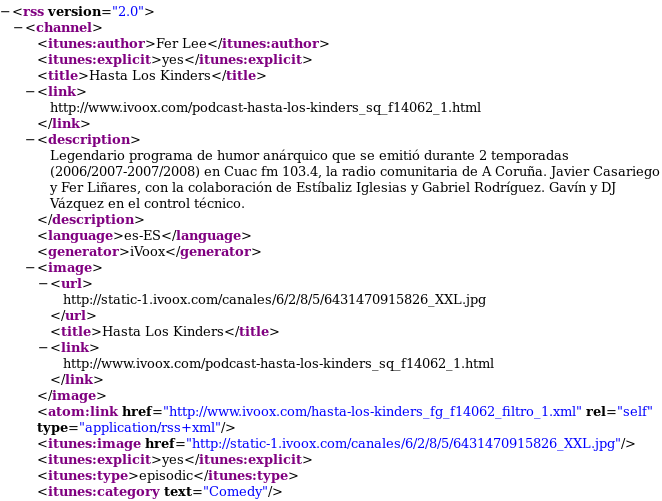
\includegraphics[scale=0.6,keepaspectratio=true]{./images/hlk_rss.png}
	\caption{Fragmento de ficheiro RSS real utilizado nas probas.}
	\label{fig:rss}
\end{figure}

RSS é un tipo de formato XML utilizado para a \say{sindicación} web, isto é, a emisión de contidos actualizados dunha páxina web a un número indefinido de subscritores. Utilízase para evitar a procura manual de novos contidos naquelas páxinas nas que a actualización é frecuente: Páxinas de novas, blogs, podcasts... 

O seu funcionamento consiste nun ficheiro RSS (comunmente chamado \say{feed}) accesible desde a web polos programas clientes de rss que posúan os subscritores. Ese feed mostra información resumida do contido publicado no sitio web ao que fai referencia. Cada vez que o contido se actualice, o feed actualizarase tamén e ese cambio será detectado polo cliente rss na súa seguinte comprobación mediante \say{polling}.
 
O nome procede do acrónimo de \say{Really Simple Syndication}(Sindicación Realmente Sinxela) e o estándar é mantido polo \say{RSS Advisory Board}. Na data de entrega desta memoria e desde o ano 2009, a última revisión é a 2.0.11 \cite{rss}

Neste proxecto, o interese céntrase na actualización dos podcasts. Existen alternativas a este formato de sindicación mais, dado o seu uso xeralizado entre os usuarios potenciais da aplicación web a desenvolver, non foron consideradas.


\subsection{JSON}

\begin{figure}[h]
	\centering
	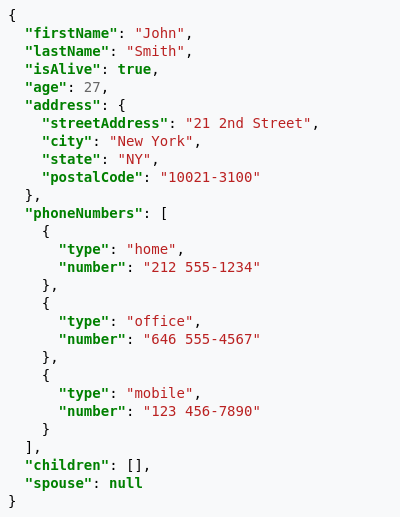
\includegraphics[scale=0.5,keepaspectratio=true]{./images/json.png}
	\caption{Exemplo de sintaxe JSON\cite{json_wiki}}
	\label{fig:json}
\end{figure}

JSON é un estándar de sintáctico utilizado para o intercambio de datos lixeiros de texto entre distintas linguaxes. A pesares de ser a abreviatura de JavaScript Object Notation pola súa orixe inspirada nos tipos desta linguaxe\cite{json} o seu uso por parte doutras tecnoloxías é común. Esta linguaxe non define un sistema completo de intercambio de datos, mais si un marco sintáctico sobre o que definir un.

Baséase nunha xerarquía definida por chaves, corchetes, comas, dous puntos e parénteses no xeito descrito na figura \ref{fig:json}, onde se amosa un exemplo de codificación dos datos persoais dun home.

Neste proxecto, utilizouse de forma implícita ao ser a codificación utilizada polos obxectos de contexto de Django.

\subsection{LaTeX}
\label{latex}

LaTeX é un sistema de preparación de documentos para os que sexa necesaria unha tipografía de alta cualidade, habitualmente, documentos medios ou longos para publicacións científicas. A motivación de LaTeX é a máxima separación posible entre o contido e o estilo do documento, facendo depender o segundo de modelos preexistentes para que os autores podan concentrarse na creación do primeiro.

Este sistema non é un editor de texto. Consiste nun conxunto de macros e un programa procesador que interpreta os mesmos. É un software libre e de código aberto (publicado baixo licenza  LaTeX Project Public License\cite{latex}). Na actualidade, pódese escoller entre distintas  distribucións libres de LaTeX que inclúen unha ampla variedade de paquetes de macros adicionais. Para a confección desta memoria, utilizouse TexLive na súa versión de 2016 por ser a máis actual dispoñible nos repositorios do Sistema Operativo no momento de comezar a escritura.






\section{Django Framework}
\label{django}
O proxecto Django nace no ano 2005 coma un conxunto de ferramentas Python para o desenvolvemento web publicadas
baixo licencia BSD. A motivación dos seus creadores, Simon Wilson e Adrian Holovaty, naquel tempo programadores
nun medio periodístico, era a homoxeneización e a reutilización de código. Isto daba resposta á necesidade de reducir
o alto custo que supón manter código ad-hoc para cada novo artigo ou función, especialmente nunha páxina que
requira unha constante actualización de contidos coma a dun diario en liña. É por iso que se adoita utilizar o 
termo \say{newsroom schedule} cando se fala da rapidez de desenvolvemento que permite o framework\cite{django1}.  

Django ofrece un conxunto de bibliotecas que dan soporte ás mecánicas máis comúns do desenvolvemento
web:

\begin{itemize}
	
	\item Persistencia: Django permite crear a estrutura da base de datos sen necesidade de escribir SQL. Isto 
	conséguese mediante a superclase Model da librería \say{db} de Django. Ao declarar unha clase de Python coma
	extensión de \say{Model}, a biblioteca ocúpase automaticamente de manter a coherencia entre as súas instancias en 
	memoria e as táboas da base de datos. 
	
	\item Peticións web: A lectura e a interpretación destas peticións son levadas a cabo polo conxunto de bibliotecas
	de HTTP do framework, encapsulando as peticións e as respostas en obxectos para formar un estándar sinxelo e garantir
	a correcta formación das mesmas.
	
	\item Enrutamento e Validación: O framework ofrece un estándar para asignar as distintas vistas definidas no código
	ás URL's desexadas. Os posibles formularios presentes nesas vistas poden ser abstraídos en obxectos de Python 
	simplificando a validación dos datos introducidos polos usuarios. A utilización destes sistemas é non obstante, 
	opcional, podendo o programador optar por utilizar sinxelos formularios HTML no caso de que isto axilizase 
	o desenvolvemento.
	
	\item Sistema para embeber datos dinámicos no HTML: O chamado \say{template system} de Django marca uns procedementos
	sinxelos para acceder aos datos xerados no código. Tamén ofrece ferramentas para implementar certa lóxica
	na presentación do front end.
	
	\item Interface de administración nativa: Por defecto, este framework dispón dun panel de administración de acceso
	reservado aos superusuarios que evita os accesos directos á base de datos no caso de que un administrador necesite
	facer cambios manuais nos datos.
	
	\item Soporte por defecto para a autenticación e autorización: Django permite ao desenvolvedor invocar a clase 
	nativa Usuario e efectuar con ela accións de rexistro, autenticación e concesión/revogación de permisos sen máis
	programación.

\end{itemize}   


Para este proxecto utilizouse concretamente Django 1.11, a versión estable máis avanzada no tempo en que se comezou o 
traballo. Django sufriu unha actualización importante desde entón que rematou coa publicación de Django 2.0 en Decembro do pasado ano 2017. Estas dúas versións non son totalmente compatibles de modo que unha actualización implicaría cambios no 
código. Tendo en conta que a Django Software Foundation, responsable do mantemento do framework, non prevee retirar o soporte á versión utilizada nun futuro próximo e que a versión de Python utilizada é soportada tamén por Django 2\cite{django2}, considerouse aceptable o grao de actualidade da tecnoloxía utilizada.    

Ademais do mencionado anteriormente, confiouse en Django para este proxecto pola súa madurez e pola súa popularidade, sendo  utilizado en sitios coma Instagram, Disqus, Pinterest ou Open Knowledge Foundation.


\section{Celery}

Celery é unha cola de traballos asíncrona baseada na mensaxería distribuída (distributed message passing). Utilízase para distribuír traballos entre máquinas ou fíos. Celery levanta un conxunto de procesos chamados \say{workers} nos que se executarán de xeito concorrente os diferentes traballos ou \say{tasks}. Eses workers consultan constantemente a cola de traballos para executar os traballos que podan estar pendentes\cite{celery}.

Neste proxecto, utilizouse Celery para controlar a execución dos demos que corren no lado do servidor. Eses dous demos son: O encargado de actualizar a información do programa e os episodios e o encargado de calcular a popularidade dos programas. Utilizouse a versión de Celery 4.1, a máis actual no repositorio de Anaconda no momento de comezar o traballo.

Django ofrece bibliotecas para traballar con Celery de xeito máis sinxelo, por exemplo, permitíndolle gardar información na base de datos do proxectos e engadindo ferramentas de administración dos procesos de Celery ao menú de administración de Django. Utilizáronse as bibliotecas django\_celery\_results 1.0.1 e django-celery-beat 1.1.1

Como xa se mencionou, Celery baséase na mensaxería, mais non inclúe un sistema de seu senón que lle hai que proporcionar un. Neste caso, optouse pola utilización de RabbitMQ (ver sección \ref{rabbit}), un dos recomendados na documentación de Celery.

\section{RabbitMQ}
\label{rabbit}

RabbitMQ é un software de \say{message passing} tipo \say{broker} mensaxes. Isto é, un sistema onde diferentes aplicacións se conectan ao broker coa fin de enviar a ou lelos deste, funcionando o dito broker coma unha cola. As mensaxes enviadas á cola por un aplicativo permanecerán aí até que sexan lidos por outro aplicativo. Unha mensaxe pode ser calquera cousa, desde meta información dos procesos até texto plano\cite{rabbitmq}.

Neste proxecto utilizouse a versión 3.6.10-1 por seres esta a máis actual dispoñible nos repositorios do Sistema Operativo no momento de comezar o traballo.


\section{Bootstrap}

Bootstrap é un framework libre e de código aberto (publicado baixo licenza MIT) para a construción de interfaces web. O Framework ofrece unha serie de modelos ou \say{templates}, cada unha cunha estrutura HTML, declaracións en CSS e, nalgúns casos, extensións JavaScript.

Neste proxecto, utilizouse a través da biblioteca de django-bootstrap4 para facilitar o uso dos elementos da versión 4 de Bootstrap desde os templates do framework de Django.


\section{Ajax}

Ajax é a abreviación de \say{Asynchronous JavaScript and XML}. Trátase dunha técnica combinada desas tecnoloxías, aínda que a miúdo substituíndo XML por JSON\cite{ajax}, utilizado para manter unha comunicación entre o lado cliente e o lado servidor nunha páxina web sen necesidade dunha recarga completa. 

Utilizando Ajax pódese facer unha petición ao servidor e recibir información de xeito asíncrono mediante JSON ou XML para, mediante a manipulación do HTML DOM con JavaScript, actualizar só partes da páxina amosada ao usuario. Utilízase para diminuír o tráfico entre os dous lados, facendo a navegación máis áxil e mellorando a interactividade.

Nesta aplicación utilizouse a través dos métodos definidos por jQuery (ver apartado \ref{jquery})

\section{Apache HTTP server}

Apache é un proxecto colaborativo para o desenvolvemento dun servidor HTTP robusto, con cualidade suficiente para o seu uso comercial, libre e de código aberto (publicado baixo licenza Apache, versión 2.0\cite{apache}). Apache implementa o protocolo HTTP/1.1 (RFC2616) xunto con varias funcionalidades frecuentemente requiridas pola web coma a personalización das mensaxes de erro (incluso mensaxes que conteñan de CGI scripts), a posibilidade de redirección e declaración de \say{alias} para as URLs de xeito ilimitado ou tamén soporte para hosts virtuais.

A pesar de que o seu dominio coma servidor máis utilizado decaeu nos últimos anos, segue a ser a opción libre máis popular, estando presente nun 36.34\% dos sitios web pertencentes ao \say{Top million busiest sites} segundo datos do mes de abril do presente ano 2018 (ver figura \ref{fig:img_netcraft}). Na actualidade é utilizado en sitios ben coñecidos coma o a páxina de novas da BBC, o sistema de pago PayPal ou a tenda de videoxogos en liña Steam\cite{netcraft}. Esta popularidade é a razón principal pola que se utilizou este software no proxecto.

\begin{figure}[h]
	\centering
	\includegraphics[scale=0.6,keepaspectratio=true]{./images/apache_graph.png}
	\caption{Cota de mercado dos servidores no Top million busiest sites (Netcraft, abril 2018)}
	\label{fig:img_netcraft}
\end{figure}

A versión utilizada foi Apache 2.4.27 por ser a máis actual no momento de comezar o traballo. Foi necesaria tamén a instalación das seguintes extensións:

\begin{itemize}
	\item Apache Portable Runtime (APR): Biblioteca que inclúe unha serie de API's para garantir o funcionamento de Apache sexa cal sexa a plataforma na que se execute. Utilizouse a versión 1.6.2 e a 1.6.0 da biblioteca complementaria APR-util. 
	
	\item mod\_wsgi: Módulo de Apache que poporciona unha WSGI (Web Server Gateway Interface), necesaria para albergar aplicativos web baseados en Python. Utilizouse a versión 4.5.17.
\end{itemize}


\section{PostgreSQL}

PostgreSQL é un sistema de xestión de bases de datos (SXBD) relacionais libre e de código aberto (Licenza PostgreSQL, permisiva) desenvolvido polo PostgreSQL Global Development Group. A linguaxe SQL soportada pretende ser o máis fiel posible ao estándar e as súas operacións cumpren coas regras ACID (Acrónimo inglés para Atomicidade, Consistencia, Illamento e Durabilidade)\cite{postgres1}. A súa orixe remóntase a 1996, polo que existe unha grande dispoñibilidade de recursos de documentación. Ese feito unido á certa experiencia persoal no seu uso xa antes de comezar o proxecto foron valorados á hora de elixir este sistema.

A versión utilizada é a 9.6-3 por ser a máis actual no momento de comezar o traballo. Para facer posible o acceso mediante Python, utilizouse o driver psycopg2 na súa versión 2.7.1


\section{Ferramentas de desenvolvemento}

\subsection{Eclipse}
\label{eclipse}

Eclipse é un IDE(Integrated Development Environment ou Entorno de Desenvolvemento Integrado), isto é, un aplicativo consistente nunha serie de ferramentas de desenvolvemento de software dispoñibles arredor dun editor de texto tales coma, por exemplo, unha consola de saída estándar e ferramentas para compilar e depurar código desde a interface proporcionada.

É principalmente empregado nos proxectos de Java, C e C++, porén, dada a súa popularidade, existen extensións dispoñibles no seu propio \say{marketpace} que nos permiten utilizalo para outras linguaxes. No caso deste proxecto, ese plugin é PyDev, que proporciona as ferramentas necesarias para o desenvolvemento non só de proxectos de Python en xeral senón especificamente de Django.

Outra extensión utilizada foi EGit na súa versión 4.8. Esta serve para manexar o control de versións  desde a interface gráfica de Eclipse. Egit utiliza JGit, unha implementación puramente Java do sistema Git (ver apartado \ref{git}).

Optouse pola versión de Eclipse máis nova no momento de comezar o traballo pese a que aínda non estaba dispoñible daquela nos repositorios do sistema operativo do equipo de desenvolvemento: Eclipse Oxygen 4.7.0. A versión de PyDev utilizada foi a 5.9.2. Valorouse PyCharm, un IDE específico para Python, coma alternativa; mais a versión de comunidade non tiña soporte para desenvolvemento específico de Django\cite{pycharm}.
 


\subsection{Git}
\label{git}

Git é un sistema de control de versións libre e de código aberto (licenza GPL v2). Un sistema de control de versións utilízase para gardar os diferentes estados (versións) do código nas distintas fases de desenvolvemento. Permite a creación de ramas para a división do traballo e de etiquetas para marcar certos hitos no proceso. Estas versións pódense gardar no equipo local ou nun repositorio remoto. No caso de Git, mantéñense copias tanto no repositorio coma nos equipos dos programadores, polo cal adoita cualificarse coma un sistema de control de versións distribuído\cite{git}.

Como se mencionou no apartado \ref{eclipse}, utilizouse sobre todo na súa implementación de EGit, mais as veces recorreuse ao paquete de sistema para realizar operacións sen necesidade de acceder a Eclipse. Neses casos, utilizouse a versión 2.9.5.

Existen outros sistemas coma, por exemplo, Apache Subversion, pero elixiuse Git pola posibilidade de publicar o código en GitHub

\subsubsection{GitHub}  

GitHub é un servizo de hosting web para repositorios de control de versións. É moi popular para o desenvolvemento colaborativo de proxectos de código aberto. Neste proxecto, utilizouse ata o momento coma alternativa gratuíta para obter un repositorio en liña pero, idealmente, tamén será utilizado para colaborar con outros desenvolvedores no futuro. 


\subsection{Dia}

Dia é un editor de Diagramas libre e de código aberto(Licenza GPL). Utilizáronse neste proxecto as súas extensións de UML para o diagrama de clases do sistema e a de Entidade Relación para o esquema de deseño da base de datos. A versión utilizada foi a 0.97.3.

Consideráronse outros editores coma, por exemplo, Umbrello, pero a elección foi DIA por criterios de estética e comodidade de uso debido á súa interface sinxela.

\subsection{Fedora}

Fedora é un Sistema Operativo que utiliza o kernel de Linux. É desenvolvido pola comunidade do Fedora Project, patrocinada desde os seus inicios por Red Hat Incorporated. Se ben as súas distintas compoñentes non están publicadas baixo a mesma licenza, estas si se enmarcan na definición de \say{Licenza de Software Libre} da FSF (Free Software Foundation) a excepción dalgúns ficheiros de firmware que, por especificación dos fabricantes de hardware, teñan que estar presentes unicamente coma arquivos binarios. Nese último caso, han de cumprimentar unha serie de requirimentos coma estar libres de pago polo seu dereito de uso\cite{fedora}. Podemos entender este, polo tanto, coma un Sistema Operativo libre.

Todo o desenvolvemento deste proxecto así coma a escritura desta memoria realizouse sobre Fedora 25 (64 bits), utilizando Xfce 4.12 coma entorno de escritorio.


\subsection{TeXstudio}

TeXstudio é un editor de documentos LaTex libre e de código aberto (Licenza GPL v2\cite{texstudio}). Proporciona, entre outras funcionalidades, un editor gráfico con soporte de marcado ortográfico para distintos idiomas, un visor de ficheiros PDF integrado e un corrector de referencias. Para este proxecto, utilizouse a versión 2.12.6 co paquete ortográfico de lingua galega de Libre Office v13-10.

Trátase unicamente dun editor, non inclúe un procesador de macros de LaTex. Utilizouse para isto a distribución TeX Live 2016 (ver sección \ref{latex}) e, para a exportación da memoria a formato PDF, pdfTex na súa versión 3.14159265 (a incluída no paquete).